\section{Synthesizing a variable solver}

\begin{algorithm}[H]
\SetAlgoLined
\KwIn{goal function $\phi$, semantic equivalence relation $=_e$, reduction order $>$, set of training expressions $E$, set of test expressions $S$}
\KwResult{a term rewriting system $R$}
\While{$\exists s \in S \st \neg \phi(s)$}{
    choose $e \in E$, $l \in \texttt{lhs\_patterns(e)}$\;
        query synthesizer for $r$ such that $l =_e r \wedge l > r$\;
    \If{$r$ is found}{
        $R \gets  R \bigcup \;\{(l \rewrites r)\}$\;
        $E \gets \{ R(e) | e \in E \wedge \neg \phi(R(e))\}$\;
    }
}
\caption{Idealized procedure for synthesizing a term rewriting system}
\label{algo:synthesis}
\end{algorithm}

Having demonstrated that we can synthesize rules to augment an existing, handwritten term rewriting system, it is natural to next synthesize a term rewriting system entirely from scratch. By back-fitting a reduction order to conform with the existing simplifier rules, we essentially derived a specification from an existing implementation (one could consider this an example of programming by demonstration, albeit one with a very large number of example programs). We define some possible reduction orders that represent strategies or gradients along which to rewrite expressions to bring them closer to the desired solved form with regard to the specified variable. We then evaluate these orders by synthesizing entirely new term rewriting systems using the orders as specifications and evaluating their performance on a suite of benchmarks.

\subsection{Rationale for synthesis pipeline}

Here we lay out the rationale for our proposed synthesis pipeline. In particular, we will discuss three key assumptions: that a reduction order can be an effective heuristic for guiding term rewrites to a desired form; that a term rewriting system can be synthesized as a series of individual rules; and that choosing candidate left-hand sides gathered from realistic inputs is an efficient means of finding rules that will have high impact on the performance of the term rewriting system.

When we specify a term rewriting system in this work, we say that it must have three properties:

\begin{itemize}
    \item it must be semantics-preserving
    \item it must terminate on all inputs
    \item it must rewrite terms into a form that has some desired property
\end{itemize}

In prior work, we showed that the Halide simplifier was semantics-preserving by verifying that for each rule $(l \rewrites r) \in R$, $l =_e r$, where the equality relation $=_e$ was checked by running the terms $l, r$ through an interpreter and sending the outputs to a solver to be checked. We showed that the TRS was terminating by choosing an order $>$ over terms and showing that every rule in $R$ rewrote terms to be strictly less in that order. When we synthesized new rules to add to the simplifier ruleset, we did not explicitly define the third criterion, but allowed the termination order fitted to the existing ruleset to guide the synthesis pipeline. 

In this section, we will define more precisely the goal or intent behind a term rewriting system. We argue that an effective means of specifying this intent for the purpose of synthesis is to use a reduction order to capture the notion of rewriting a term to be closer to some goal state.

\begin{figure}
    \centering
\subfigure[$\termlang$]{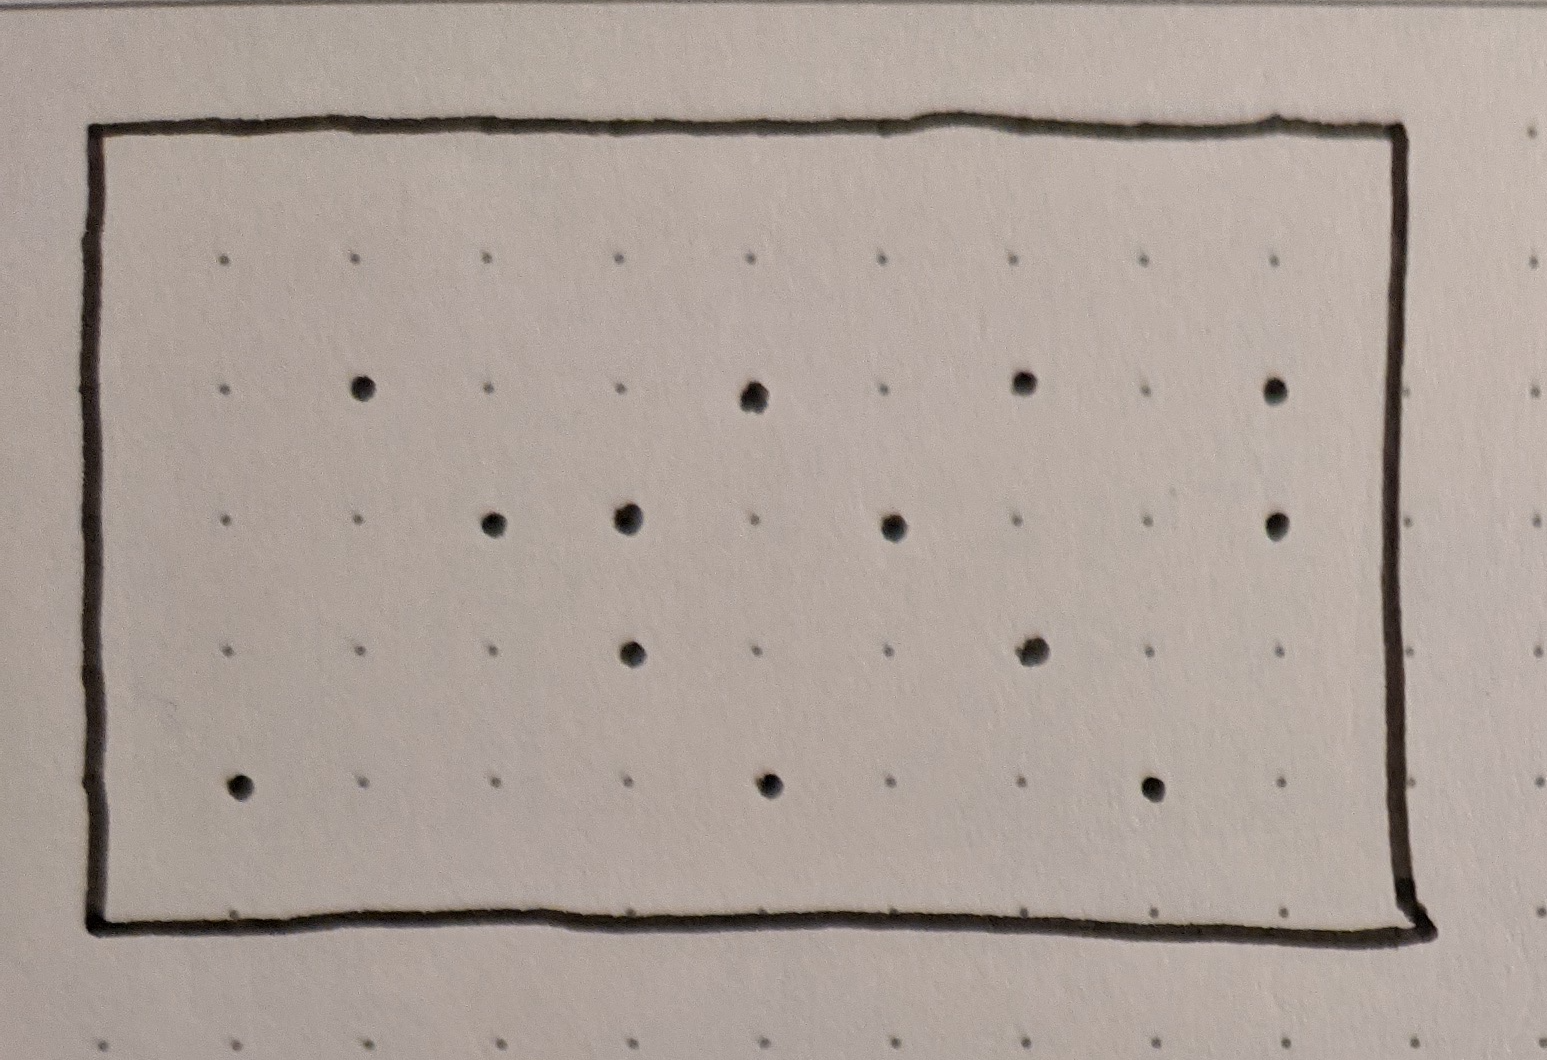
\includegraphics[width=0.3\textwidth]{figures/diagram1.png}}
    \hspace{1em}
    \subfigure[$\{s | s \in \termlang \wedge \phi(s)\}$ in red]{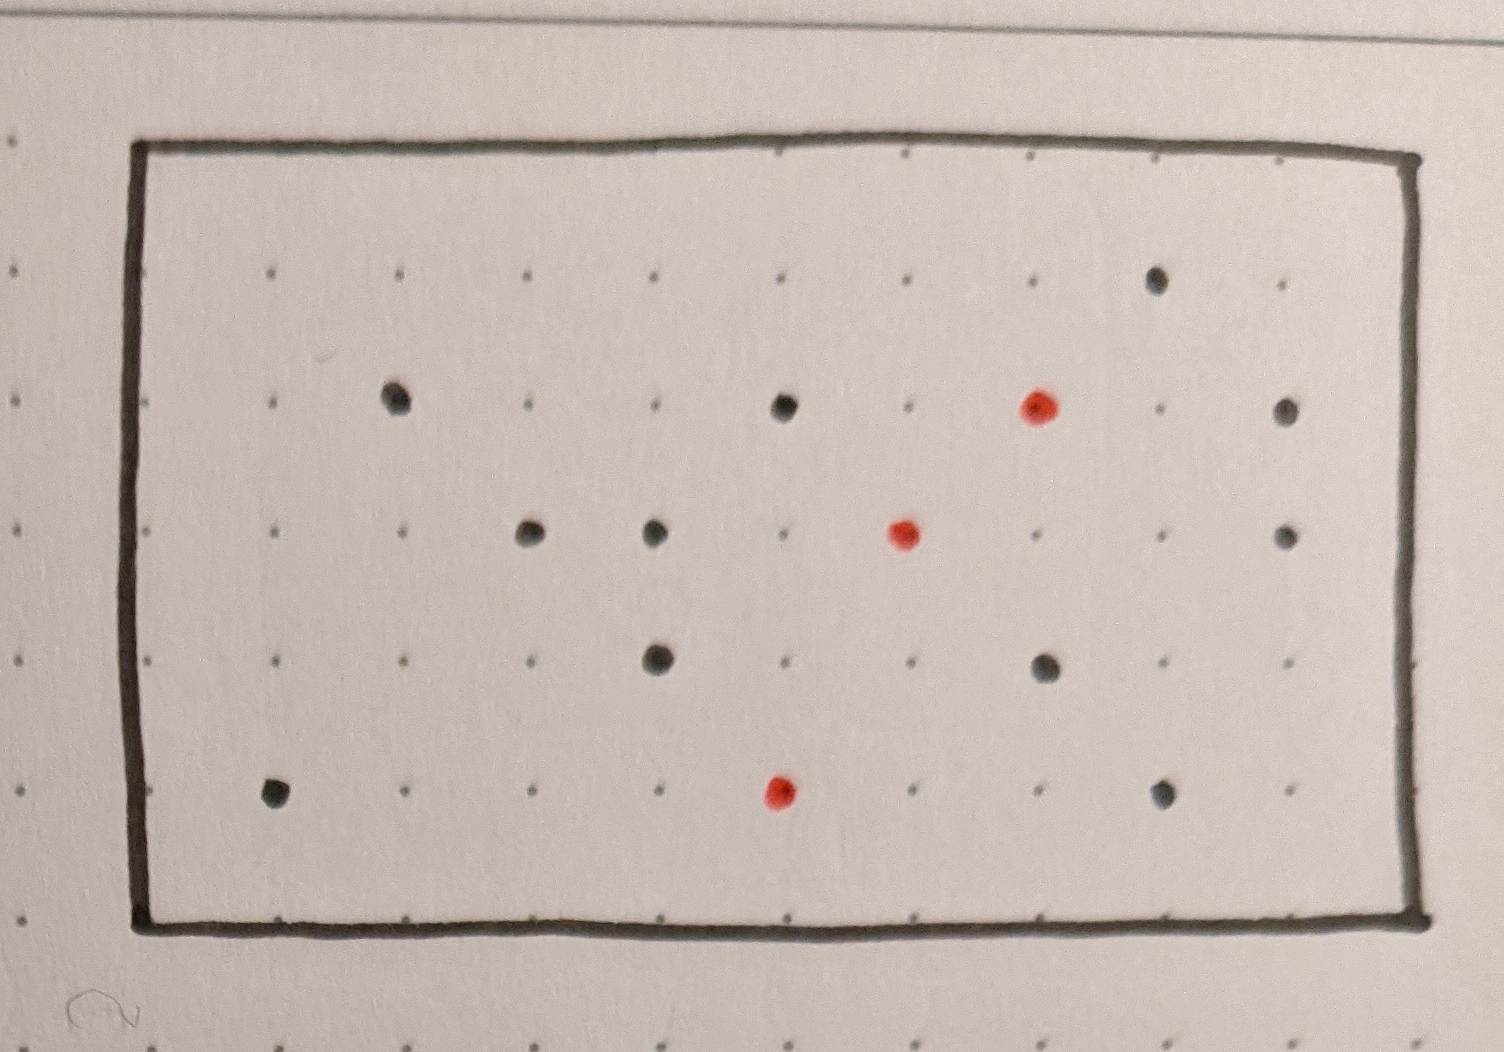
\includegraphics[width=0.3\textwidth]{figures/diagram2.png}}
    \hspace{1em}
    \subfigure[$\goallang$ in blue]{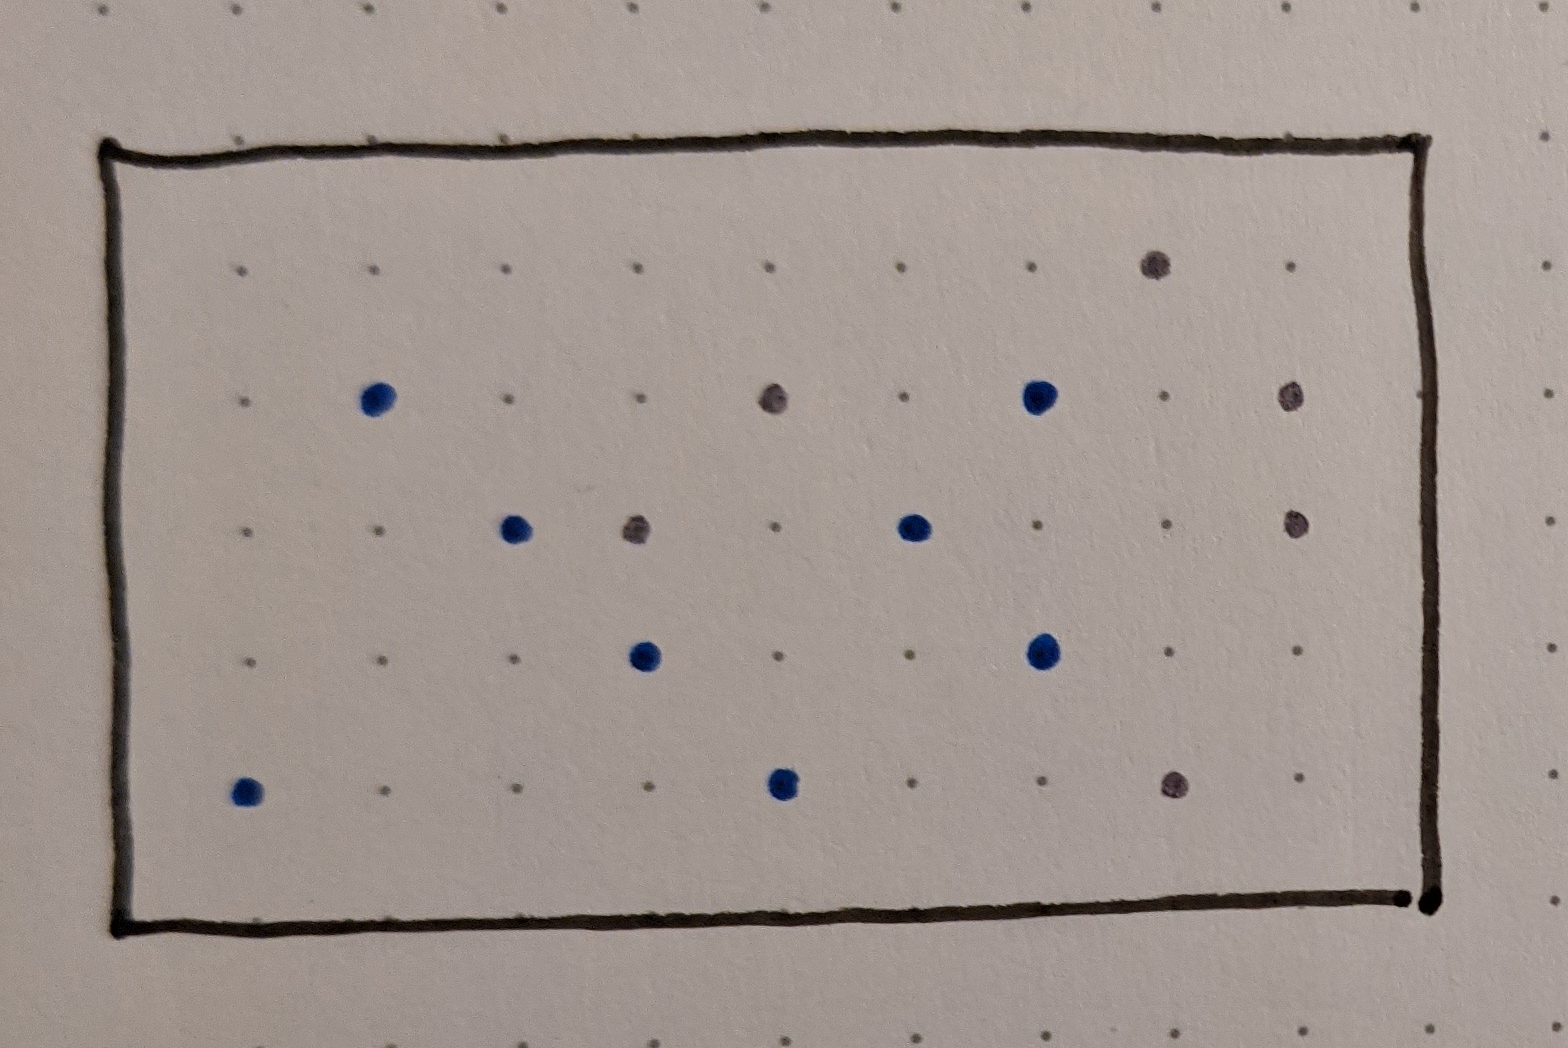
\includegraphics[width=0.3\textwidth]{figures/diagram3.png}} \\
    \subfigure[Undirected edges connect all $s, t$ st. $s =_e t$]{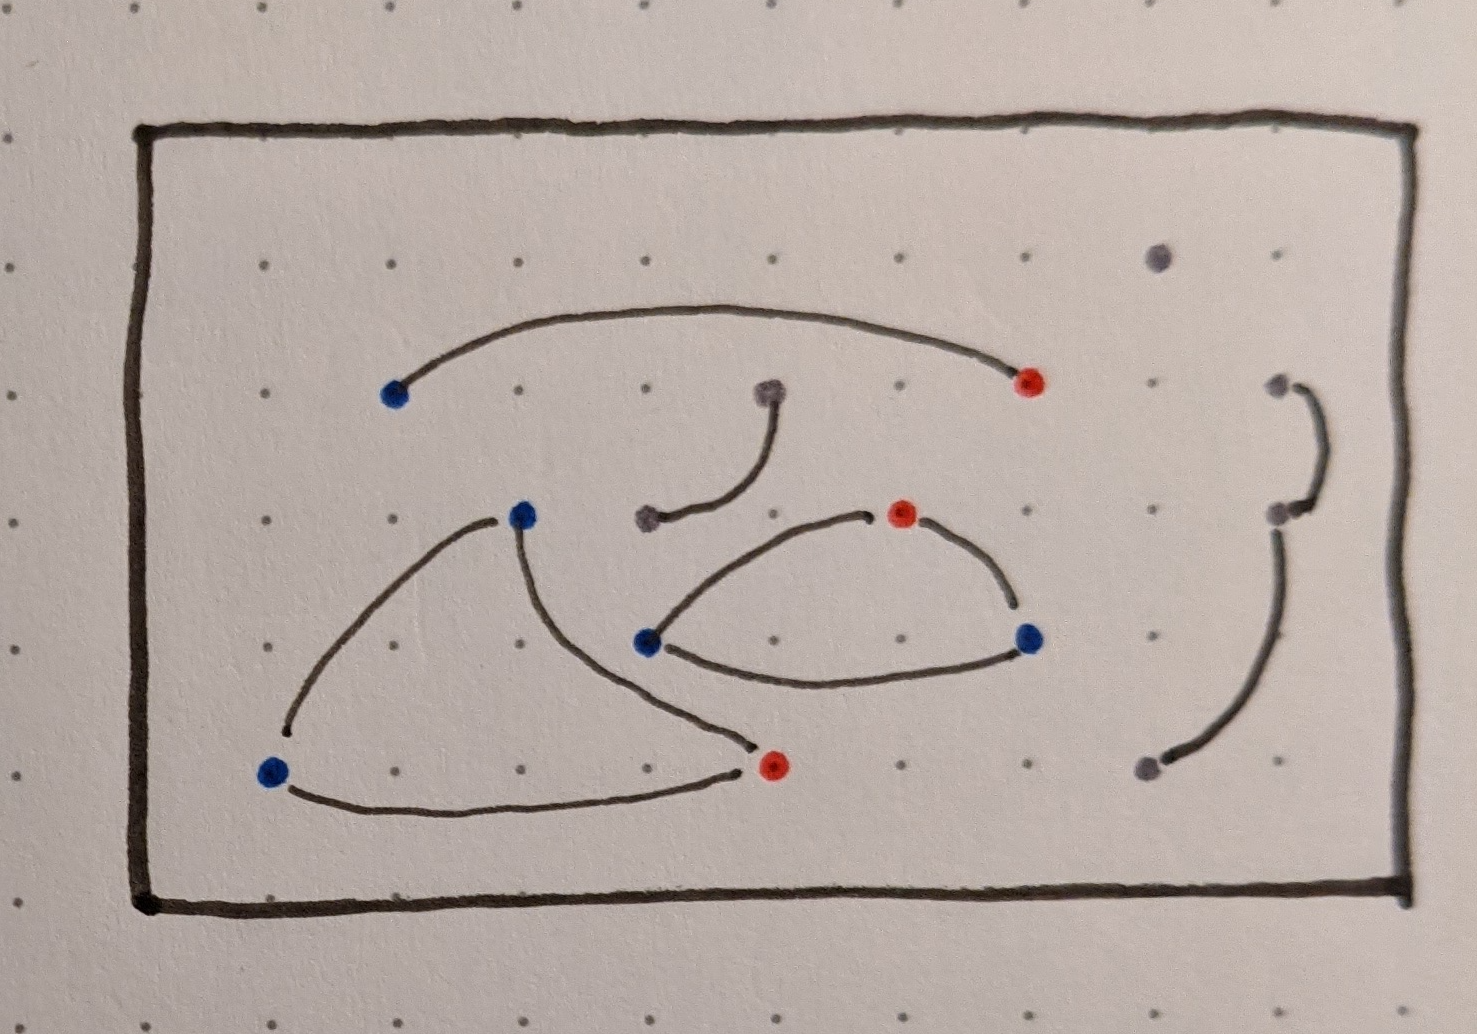
\includegraphics[width=0.3\textwidth]{figures/diagram4.png}}
    \hspace{1em}
    \subfigure[Directed edges connect all $s, t$ st. $s =_e t \wedge s > t$]{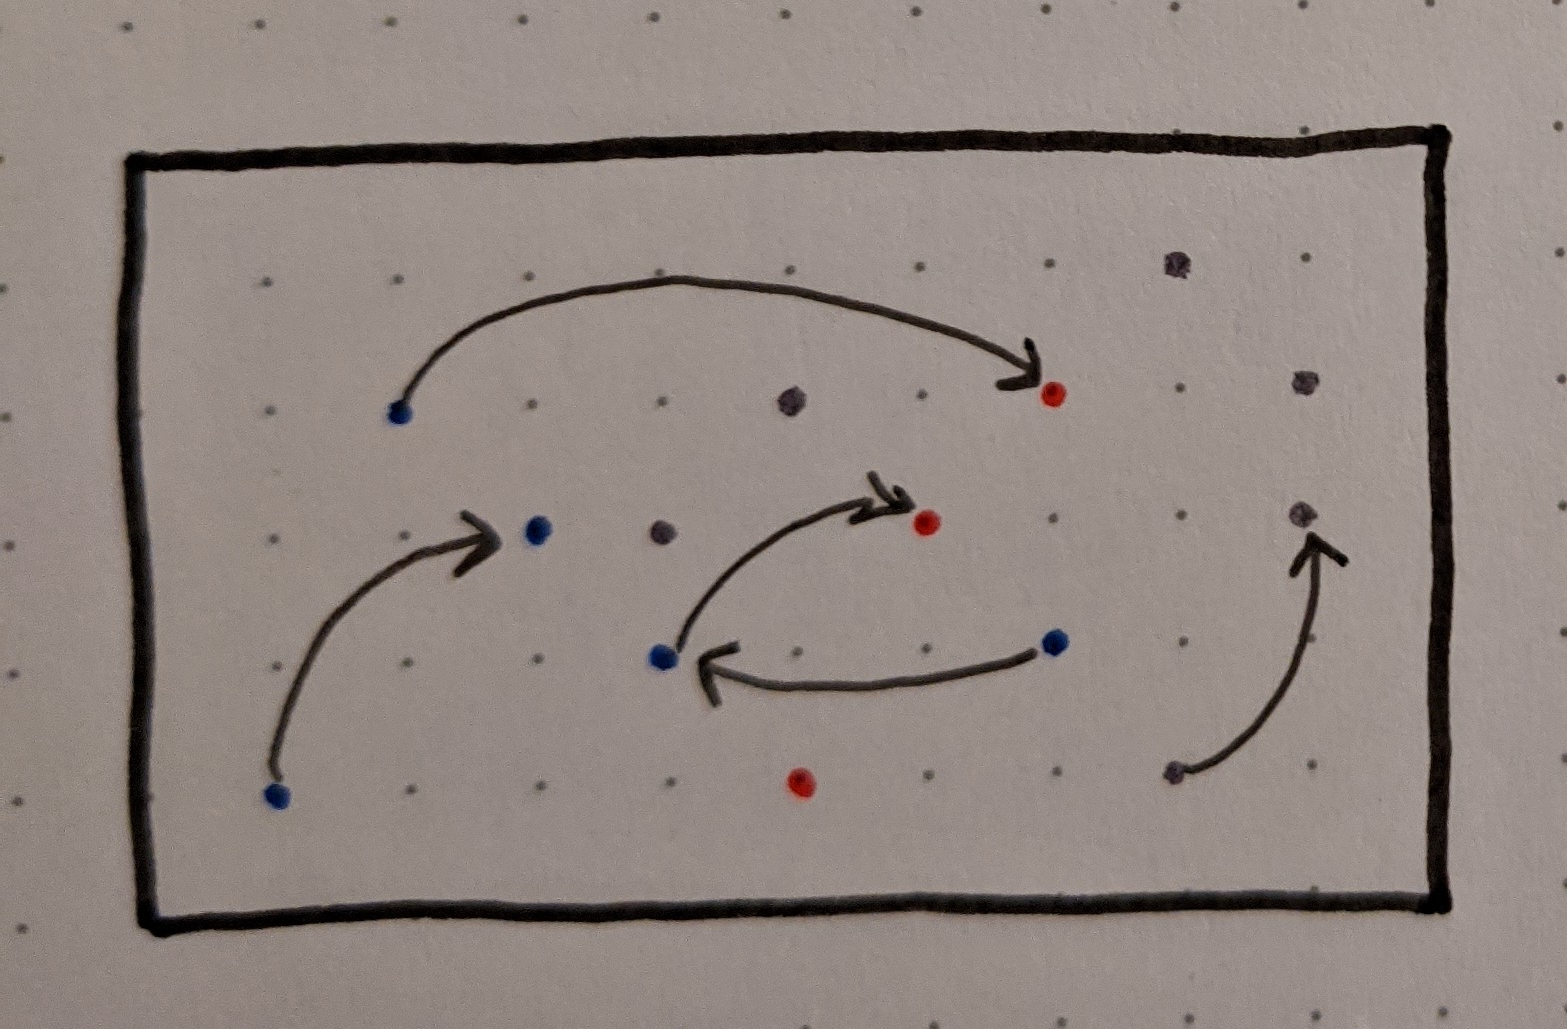
\includegraphics[width=0.3\textwidth]{figures/diagram5.png}}
    \caption{Each dot in (a) represents a term in $\termlang$. In (b), each term in the goal state is drawn in red. In (c), all terms which are equivalent to a term in the goal state ($\goallang$) are drawn in blue. The goal of the term rewriting system is to rewrite all blue dots in (c) to a red dot in (b). In (d), undirected edges connect all pairs of terms that are semantically equivalent. In (e), those edges have been oriented with a reduction order. Given the specification $\forall (l \rewrites r) \in R \st l =_e \wedge l > r$, we can find a TRS $R$ by picking a finite subset of all the directed edges in (e).}
    \label{fig:termuniverse}
\end{figure}

First, we define the goal property that describes the underlying intention of the term rewriting system. Assume some language of terms $\termlang$, a semantic equivalence relation over those terms $=_e$, and a syntactic equivalence relation $=$. We write the goal property as a predicate function $\phi$ such that $\phi(s)$ is true if $s$ is in the goal state and false otherwise. We can thus write the domain of the term rewriting system as a language $\goallang \subseteq \termlang$, defined as

\[
\goallang = \{s | s \in \termlang \wedge (\exists t \in \termlang\;.\; s =_e t \wedge \phi(t))\}
\]

We want our term rewriting system to put every term in $\goallang$ into a form that satisfies our goal function $\phi$. It doesn't matter what the term rewriting system does to terms which are in $\termlang$ but not $\goallang$ so long as it obeys the semantics-preserving and termination properties.\footnote{We might prefer that the term rewriting system act on terms not in $\goallang$ as little as possible, but this is purely for performance reasons and can be set aside for now.}

As two running examples, let us consider two term rewriting systems that represent different aspects of the Halide simplifier TRS. As in the rest of this work, we assume that $\termlang$ is the Halide expression grammar. First, we consider a prover TRS, which tries to determine if an expression is equivalent to the booleans values true or false, or if its truth value is unknown. We state that the prover has a domain language $\goallang_P$ and a goal state function $\phi_P$ such that

\begin{align*}
    \goallang_P = \{s | s \in \termlang \wedge (s =_e \htrue \vee s =_e \hfalse)\} \\
    \phi_P(s) := s = \htrue \vee s = \hfalse
\end{align*}

The second example is a TRS that seeks to show that a given expression is monotonic. The goal function for this TRS is a bit more subtle. The Halide compiler's means of querying the monotonicity of an expression is sound but not complete: it walks the expression to see if it is in a syntactic form that can be recognized as monotonically increasing, monotonically decreasing, or constant. If it cannot recognize the expression as any of these three, it returns unknown. The job of the monotonic rewriter TRS is to put expressions into this syntactic form wherever possible. We say then that the domain language of the monotonic rewriter $\goallang_M$ is all terms $s$ in $\termlang$ where there exists some term $t$ such that $s =_e t$ and $t$ is in a syntactic form that can be recognized as monotonic or constant by the function $\texttt{is_monotonic}$ in the Halide codebase. The goal state function $\phi_M$ returns false when $\texttt{is_monotonic}$ returns unknown on an input term, and true otherwise.

We write $R(s)$ for the output of a term rewriting system $R$ on the input term $s$. Assume we use the means of assuring semantics preservation and termination as used above. Then, for an equivalence relation $=_e$ and a goal function $\phi$, we write that a specification for an ideal TRS $R$ thus:

\begin{align*}
\forall s \in \goallang \st \phi(R(s)) \wedge \\
\forall t \in \termlang \st t =_e R(t) \wedge R(t) \textrm{ terminates }
\end{align*}

Of course, since our theory is undecidable, the $\forall s \in \goallang \st \phi(R(s))$ portion of our specification is almost certainly unrealizable in the general case. Instead, we would like to encode a means of making progress towards this goal, rather than ruling out all TRSs that do not achieve it. We can think of this as a strategy for rewriting terms to be closer to the desired goal state. For example, imagine we started writing rules for the prover, and started with this pair:

\begin{align*}
    x = x \rewrites \htrue \\
    x + (y - y) \rewrites x
\end{align*}

We might note that the second rule is canceling like terms, and add many more rules that do the same. If we wanted to formally encode this strategy, we could do so using an order over terms, such that terms that satisfy the goal condition $\phi$ would be least elements in that order. In the case of the prover, the order could be to compare terms by their length; since the boolean constant $\htrue$ is of the shortest possible length in the Halide expression language, it is a least element of this order. Let us call such an order $\goalorder$ and add it as a condition to our specification:

\begin{align*}
\forall s \in \goallang \st \phi(R(s)) \wedge  s \geq_{\phi} R(s) \wedge \\
\forall t \in \termlang \st t =_e R(t) \wedge  R(t) \textrm{ terminates }
\end{align*}

As pictured in figure~\ref{fig:termuniverse}, the process of choosing rewrite rules for a ruleset is choosing edges from the graph (d) and orienting them. The goal order $\goalorder$ could be considered an order traversal from terms not in the goal state to terms that are. 

Now, assume we have been given some solution to our specification in the form of a term rewriting system $R$. How can we prove that it fulfills our criteria? In prior work, we proved that a term rewriting system was semantics-preserving ($\forall t \in \termlang \st t =_e R(t)$) and terminating ($\forall t \in \termlang \st R(t) \textrm{ terminates }$) by showing that those properties held over every rule in the ruleset. We can use a similar strategy here: if the goal order $\goalorder$ holds for every rule in $R$, then it must hold for all of $R$ as a whole.

\begin{assumption}
We can lower our requirement that the ruleset $R$ rewrite every term in $\goallang$ to the goal state to the requirement that every rule in $R$ rewrites terms to be closer to the goal state, as described by a goal order $\goalorder$.
\end{assumption}

% describe this more clearly: 
Requiring the goal order hold over every rule in $R$ will exclude some possible term rewriting systems for which the goal order would hold over the full system, just as requiring that the termination property hold over every rule in $R$ excludes some TRSs that are terminating. This is illustrated in figure~\ref{fig:termuniverse}; when we choose an order that turns the undirected edges in (d) to directed edges in (e), there are now some terms in $\goallang$ that are unable to reach a goal state. However, checking that this property holds over every rule can be done quickly and automatically. Just as with the termination guarantee, so long as every rule we add to a ruleset conforms to the goal order, we can add, delete, or permute the priority of rules without fear of losing our overall guarantee. This quick machine-checkable proof allows us to synthesize a TRS without human supervision.

In order for the goal order to hold over every term that may match and be rewritten by a rule, it must be a valid reduction order: well-founded, $\Sigma$-operation compatible, and closed under substitution (see~\cite{baader1999term}). Usefully, this means we do not need a separate termination order; since a goal order requires that each rewrite moves a term monotonically lower in the order, it also provides a termination guarantee.

We can now restate our term rewriting system specification like so:

\begin{align*}
    \forall s \in \goallang \st \phi(R(s)) \wedge \\
    \forall (l \rewrites r) \in R \st l =_e r \wedge l \goalorder r
\end{align*}

Since any term rewriting system we wish to synthesize will be semantics-preserving, the major decision we need to make in specifying a term rewriting system is to pick a goal order:

\begin{assumption}
We can effectively formalize the goal of a term rewriting system by choosing a \emph{goal order} over terms such that, for two terms $s$ and $t$ such that $s \goalorder t$ in this order, $t$ is assumed to be closer to the goal state.
\end{assumption}

Finding a goal order that encodes progress towards a goal state is a difficult task, and requires human intuition and ingenuity. Our work does not directly aid in this task, which is still up to the human author of the term rewriting system; however, our synthesizer machinery can aid in experimenting with and selecting goal orders.

\begin{table}[]
    \centering
    \begin{tabular}{|l|l|l|}
    \hline 
        TRS & Goal function $\phi$ & Goal order $>$ \\
        \hline 
        Prover &  $\phi(s)$ if $s$ is $\htrue$ or $\hfalse$ & $s > t$ if $t$ is shorter than $s$\\
        \hline
        Monotonic rewriter & $\phi(s) := \texttt{is_monotonic(s)}$ & $s > t$ if $s$ has more $\%$ ops \\
                 & & $s > t$ if $s$ has more constants \\
        \hline
    \end{tabular}
    \caption{Two term rewriting systems, goal functions that encode their intent, and goal orders that represent moving towards those goals}
    \label{tab:trsspecs}
\end{table}

As discussed above, the prover could adopt a strategy of making expressions shorter, with the aim of eventually being able to reduce them to the constants $\htrue$ or $\hfalse$. For the monotonic rewriter, one expression in the goal state is $x \cdot c_0$ where $c_0$ is a positive constant; the monotonicity checker recognizes this form as monotonically increasing. So, one possible strategy could be to move constants to the right side of an equation wherever possible. We may also want to employ sub-strategies: if the prover TRS contains the rule $x = x \rewrites \htrue$, we might choose a strategy of putting expressions into a kind of canonical form wherever possible, so we can rewrite an expression $e_1 = e_2$ into $e' = e'$ and then apply the identity rewrite rule. The simplifier reduction order, which was composed of several orders lexicographically, could be said to employ a series of sub-strategies in this way. See table~\ref{tab:trsspecs} for the prover and monotonic rewriter goal functions and some goal orders that approximate them.
 % check with Andrew about monotonic rewriter example

If we accept the assumption that a reduction order can encode the strategy of rewriting a term to be closer to our goal, we now have a specification that should hold for every individual rule we synthesize:

\[ \forall (l \rewrites r) \in R \st l =_e r \wedge l \goalorder r
\]

The set of possible rules made up of terms in the Halide expression language that conform to that spec is still infinitely large. The other part of our spec required that $\forall s \in \goallang \st \phi(R(s))$, but this is unrealizable. Instead we relax to a specification that could actually be checked; for example, we could fix a set $S$ of terms and write that our term rewriting system should:

\begin{align*}
    \forall s \in S \st \phi(R(s)) \wedge \\
    \forall (l \rewrites r) \in R \st l =_e r \wedge l \goalorder r
\end{align*}

Now we have a realizable synthesis procedure: we can synthesize rules $(l \rewrites r)$ such that $l =_e r \wedge l \goalorder r$, add them to $R$, and terminate when $\forall s \in S \st \phi(R(s))$ holds, as described in algorithm~\ref{algo:synthesis}. In practical cases, we may want to use other termination conditions, such as requiring that some fraction of $S$ can be solved. In our prior work, we did not check that the outputs of the synthesis-augmented simplifier brought previously unsolved terms to the goal state at all, but relied on a fairly complex goal order to produce a strengthened ruleset that was demonstrably more effective on our benchmarks.

Finally, we need a strategy for choosing which rule to add to growing ruleset at each step. As the space of potential rules is so large, even if term sizes are bounded, simply sampling at random may not be effective. Our synthesis pipeline defines a strategy for growing a ruleset so that it is able to rewrite more and more of $\goallang$, in a way that is of practical benefit to the compiler. In prior work, we gathered a corpus of expressions seen by the compiler in realistic circumstances and mined them for general patterns to form candidate LHS terms. We then attempted to synthesize RHSs for each candidate LHS term to form rules. We assert that this is an effective method of creating a ruleset is effective under realistic workloads.

\begin{assumption}
An effective heuristic for choosing candidate left-hand side terms for new rules is to gather expressions seen by the compiler under realistic circumstances and mine them for general patterns.
\end{assumption}

Note that when we gathered input expressions in prior work, we did not check to see if those expressions were in the TRS domain $\goallang$. Any means of checking membership in $\goallang$ is necessarily incomplete, so any ruleset learned from a checked input list would inherit the incompleteness of the checker. Also, note that we will want to rewrite subterms of expressions that are not themselves in $\goallang$: in the prover TRS, although all input expressions are boolean-valued, we will want to rewrite subterms of all possible types. For example, given the ruleset $R = \{x = x \rewrites \htrue, x + x \rewrites x \cdot 2\}$, we need the second rule that rewrites a numeric-valued expression so that we can rewrite $x + x = x \cdot 2$ to $\htrue$.

Given these three assumptions, we propose the synthesis pipeline in algorithm~\ref{algo:synthesis}. 

\subsection{The Halide variable solver}

The Halide simplifier was a fairly mature system, in production for over a year and consists of almost a thousand rules. The Halide variable solver, by contrast, is a much smaller system, currently implemented as a series of if statements rather than a formal term rewriting system, and consisting of the equivalent of less than a hundred rules. The simplifier's use cases were quite varied and complex, and the existing ruleset required a complex composite reduction order to cover their full purpose. The variable solver is much smaller and more focused and can be captured by much simpler reduction orders. With the variable solver, therefore, we have the opportunity to experiment with various reduction orders to find the one that fulfills the system's purpose best, and to synthesize a TRS entirely from scratch, rather than augment an existing system.

% synthesis pipeline: Rosette, encoding reduction order as metasketches, metasketch search order, etc
% discussion of different granularities of reduction order
% evaluation of various synth'd TRSs

\section{The variable solver reduction orders}

Here we refer to \emph{target-matching variables} as variables that can be unified with the target variable or subterms that contain the target variable. Variables that cannot be unified with the target variable or subterms that contain the target variable are called \emph{non-target-matching variables}. All variables that occur in the variable solver ruleset are either target-matching or non-target-matching. Allowing variables that can match either target variable-containing subterms or non-target variable containing subterms complicates reduction order definitions. \jln{is it true that any rule containing variables that can match anything can be replaced by multiple rules that only contain target-matching or non-target-matching variables?}

We represent target-matching variables as $x^t, y^t$, etc., and non-target-matching variables as $x^n, y^n$, and so on.

\subsection{Reduce occurrences of target-matching variables}

\[ s_1 >_t s_2 \iff \forall x^t \in \mathcal{V}(s_1) |s_1|_{x^t} \geq |s_2|_{x^t}
\]

The proof that this order is a valid reduction order is straightforward. The order is clearly well-formed, since $|s|_{t_i}$ has a minimum value of 0. The order is compatible with $\Sigma$-operations; for any

\[ s_1 >_t s_2 \implies f(t_1,...t_{i-1},s_1,t_{i+1},...,t_n) >_t f(t_1,...t_{i-1},s_2,t_{i+1},...,t_n)
\]

\begin{align*}
\sum_{x^t \in \mathcal{V}} \sum_{0}^{i - 1} |t_k|_{x^t_k} + |s_1|_{x^t_k} + \sum_{i + 1}^{n} |t_k|_{x^t_k} >
\sum_{x^t \in \mathcal{V}} \sum_{0}^{i - 1} |t_k|_{x^t_k} + |s_2|_{x^t_k} + \sum_{i + 1}^{n} |t_k|_{x^t_k}
\end{align*}

Since $|s|_{x^t}$ is always non-negative, the implication clearly holds.

Finally, the order is closed under substitutions. A substitution $\sigma$ could increase the number of target-matching variables in $s_2$ by replacing some $x^t$ with a subterm containing multiple target-matching variables, but since all target-matching variables in $s_2$ must occur an equal or greater number of times in $s_1$, the order must be preserved. Any substitution for a non-target-matching variable will have no effect on the number of target-matching variables in $s_1$ or $s_2$ by definition. 

Note that this order does not require that the number of non-target-matching variable occurrences in $s_1$ be equal or greater to the number of occurrences in $s_2$; it is perfectly fine to increase the size of the rewritten expression so long as the count of target-matching variables goes down. \jln{put example here}

\subsection{Move occurrences of target-matching variables to the left}

The intuition behind the order is simple, but we will have to take care in our definition to make sure it is a valid reduction order. We define this order by transforming terms into strings and then comparing the strings lexicographically.

To transform a term into a string (we write this function as $\texttt{varstr}(s)$), we first take the sequence of all occurrences of variables and constants in the term, in the order in which they occur. We truncate the sequence by removing everything after the last occurrence of a target-matching variable. We then replace all target-matching variables with 'a' and all non-target-matching variables or constants with 'b', and compare the resulting string with that of another term in lexicographic order (such that a $<$ b).

\begin{tabular}{llll}
$n_0 + t_0 $>$ t_0 + n_0$ & $(n_0 t_0) > (t_0 n_0)$ & $(n_0 t_0) > (t_0)$ & ab $>$ a \\
\end{tabular}

This order is clearly compatible with $\Sigma$-operations; if $\texttt{varstr}(s_1) > \texttt{varstr}(s_2)$, then the order will still hold if identical prefixes and suffixes are added to both terms. However, we need to add an additional condition to make the order closed under substitution. Consider a rule

\[ (n_0 + n_1) + (t_0 + n_2) \rewrites (n_2 + t_0) + (n_0 + n_1)
\]

The rule appears to move the target-matching variable to the left and thus seems to be in conformance with the order. However, given the substitution $\sigma = \{ n_0 \mapsto y^n, n_1 \mapsto z^n, t_0 \mapsto x^t, n_2 \mapsto ((u^n + v^n) + w^n)\}$, we obtain the transformation
\[ (y^n + z^n) + (x^t + ((u^n + v^n) + w^n)) \rewrites (((u^n + v^n) + w^n) + x^t) + (y^n + z^n)
\]

which actually shifts the target-matching variable to the right.

To disallow this ordering, we add the condition that a rewrite rule that follows this order cannot permute the sequence of target-matching variables or the sequence of non-target-matching variables; it can only change how the two sequences are interleaved. In the example above, the sequence of target-matching variables is unchanged between the two terms, but the sequence of non-target-matching variables has been reordered.

\begin{tabular}{ccccccccc}
      &       & $t_0$ &       & $\rewrites$ &       & $t_0$ &       & \\
$n_0$ & $n_1$ &       & $n_2$ &             & $n_2$ &       & $n_0$ & $n_1$
\end{tabular}

Similar issue if we are allowed to reorder target-matching variables

\[ (t_0 + n_0) + t_1 \rewrites (t_1 + t_0) + n_0
\]

\[ \sigma = \{ t_0 \mapsto x^t, n_0 \mapsto y^n, t_1 \mapsto ((z^n + w^n) + x^t)\}
\]

\jln{finish proof and write formal definition of order}

\subsection{Move occurrences of target-matching variables up}
\jln{formally define order and prove it is a valid reduction order}

\subsection{Put rewritten expression into fully solved form}

\jln{formally define order and prove it is a valid reduction order}

\section{The synthesis algorithm}

How the Rosette synthesis procedure works

Strategy for prioritizing the search space: sorting input expressions by size, choice of LHS from a given input expression, choice of sketches

Encoding reduction orders as metasketches

\section{Evaluation of synthesized TRSs}

Evaluate synthesized TRSs on set-aside input expressions, against performance of handwritten solver.

Put into Halide compiler and see if any difference on compiled pipelines is observable.


\section{Related work}
\label{sec:related}

Perhaps the closest related work is the Alive project~\cite{lopes2015alive,menendez2017aliveinfer}.
The fundamental difference between Alive and this
work is that Alive works within the decidable theory of bitvectors, while
(because of Halide semantics) we must use the undecidable theory of integers;
this constraint is the major reason for many of our design choices. In addition:
Alive verifies optimizations (and Alive-Infer synthesizes preconditions), while
we synthesize rewrites and predicates, as well as verify them; Alive must contend
with more types of undefined behavior, which the Halide expression
language need not consider; and Alive uses a simple reduction order in
which all optimizations reduce program size, while our termination proof is more
complex. We originally tried synthesizing rule predicates with the approach used
by Alive-Infer but were not successful: using Z3 to generate positive and
negative examples did not scale for us, requiring seconds to minutes per query
due to the underlying theory of integers.  Moreover, queries with
division/modulo over the integers often did not work at all, simply returning
``unknown.''

Most recently, leveraging a TRS along with synthesized rules has been applied
to optimizing fully-homomorphic encryption (FHE) circuits~\cite{lee2020fhe}.  This
system synthesizes equivalent circuits with lower cost from small example circuits,
then applies the equivalences in a divide-and-conquer manner; the rewrites do
not contain preconditions. In further contrast to our work, the domain of FHE yields a
simple cost function (the depth of nested multiplications in the circuit), and
the underlying theory of boolean circuits is decidable.

Herbie~\cite{panchekha2015automatically}, a tool for improving the accuracy of floating point arithmetic, uses an egraph term rewriting system made up of a small library of axioms to find repairs once a fault has been localized. Herbie assures termination by bounding the number of rewrites their system may apply, and achieves good performance by pruning the expression search space and applying rewrites only to particular expression nodes. 

Besides the closely-related projects described above, program synthesis has been applied to term rewriting systems in several domains. Swapper~\cite{singh2016swapper} synthesizes a set of rewrite rules to transform SMT formulas into forms that can be more easily solved by theory solvers, similar to the use of the Halide TRS as a simplifier, using the SKETCH tool. \citet{butler2017synthesizing} learns human-interpretable strategies (essentially rewrite rules) for puzzle games such as Sudoku or Nonograms and \citet{butler2018framework} finds tactics for solving K-12 algebra problems, both using a CEGIS loop similar to our synthesis process. None of these address termination, although Swapper likely screens out non-terminating rulesets through its autotuning step. The Butler works both focus on synthesizing small, highly general rulesets that are similar to human rewriting strategies, unlike the Halide TRS which tolerates very large rulesets.  The \textbf{$\lambda^2$} tool~\cite{feser2015lambda} for example-guided synthesis performs inductive synthesis from examples, using a combination of inductive and deductive reasoning combined with enumerative search.  While our rewrite rules do not have the benefit of examples, it may be possible to apply this technique to obtain more sophisticated predicate synthesis for our rewrites.

Superoptimization, a process of finding a shorter or more desirable program that is semantically equivalent to a larger one, is similar to our work synthesizing right-hand side terms for candidate LHSs. STOKE~\cite{schkufza2013stochastic} uses Monte Carlo Markov Chain sampling to explore the space of x86 assembly programs, while \citet{phothilimthana2016scaling} describes a cooperative superoptimizer that searches for better programs using multiple techniques in a way that allows them to learn from each other.  Souper~\cite{sasnauskas2017souper} is a recent synthesis-based superoptimizer for LLVM, which was used in evaluating the effectiveness of Alive-Infer's{} precondition synthesis.

PSyCO~\cite{lopes2014weakest} synthesizes preconditions that guarantee a compiler optimization is semantics-preserving, using a counterexample-driven algorithm similar to our rule CEGIS loop (although not like our predicate synthesis algorithm). PSyCO finds the weakest precondition from a finite language of constraints, while the space of our predicate search is theoretically inifinite but in practice bounded by our iteration limit. PSyCO must reason about side effects by tracking read and write behavior in optimization templates, while our expression language is side effect--free. More recently, Proviso~\cite{astorga2019learning} finds preconditions for C\# programs using an active learning framework composed of a machine learning algorithm for decision trees as a black-box learner and a test generator that acts as a teacher providing counterexamples. Like this work, the logic of preconditions they synthesize is in an undecidable domain.

Other software that can solve equations in the manner of the Halide variable solver include SymPy~\cite{10.7717/peerj-cs.103}, MATLAB~\cite{higham2016matlab}, and GNU Octave~\cite{eaton1997gnu}. We plan to benchmark various synthesized versions of the Halide variable solver against these tools. 